\chapter{Marco Teórico}


El proyecto es un sistema interactivo que busca proporcionar al usuario independientemente de sus intereses, el cumplimiento de sus expectativas, siendo un desarrollo a conciencia, pero sin tomarlo demasiado en serio, busca también romper el estereotipo que imponen los proyectos de esta modalidad, que si bien, ofrecen un producto de relativa buena calidad y mantenimiento, son o bien productos comerciales como es el caso de Just Dance o productos privatizados como son los desarrollados para la medicina. 

En cambio, se tiene la expectativa de ofrecer al nivel de Open source del proyecto, que a la larga atraiga a más miembros, al igual que Linux o Apache y pueda expandir sus horizontes y calidad del producto, teniendo presente que Open Source no significa simplemente compartir el acceso al código fuente, como indica la \href{https://opensource.org/docs/definition.html}{Open Source Definition (OSD)}. 

El desarrollo del proyecto empleara los recursos disponibles y al alcance de cualquier desarrollador, por tanto, no tomara en cuenta el manejo de cámaras de profundidad, esta aclaración es necesaria, ya que la calidad del producto final puede ser muy variable al de proyectos similares y es una característica más por la que sobresaldría este proyecto, ya que reduciría el presupuesto necesario para el consumidor.\\

A continuación, se debe mencionar factores importantes sobre la implementación del proyecto, como las propiedades del Body Tracking, la verdadera forma que tiene esta herramienta que tiene para ofrecer al software, por que no sobra mencionar las distinciones entre una cámara normal y una de profundidad.


\section{Body Tracking/Motion Capture}

El seguimiento corporal del cuerpo, normalmente conocido como Body Tracking o Motion Capture hace referencia al seguimiento del cuerpo humano a través de una cámara, existen dos acercamientos a este estudio, el enfoque de ajuste del modelo y el enfoque de aprendizaje. El enfoque de ajuste del modelo involucra ajustar el modelo formulado según imágenes previas cargadas, estimando parámetros de puntos especificados de la imagen, sin embargo, es demasiado dependiente de extremos locales y la inicialización adecuada, lo cual lo vuelve inservible en ambientes nuevos. Este modelo comparte una similitud al método Monte Carlo basados en cadenas de Markov \cite{siddiqui2010human}.

En cambio, el enfoque de aprendizaje requiere de grandes cantidades de imagenes con notas y especificaciones del esqueleto en las imagenes, incrementando las dimensiones de espacio y memoria requerido. Un ejemplo de este tipo de reconocimiento es la herramienta PoseNet, derivado de TensorFlow, empleado para identificar objetos a partir de una base de datos propia que clasifique los elementos que se buscan identificar con silueta y nombre.

\begin{figure}[t!]
	\centering
	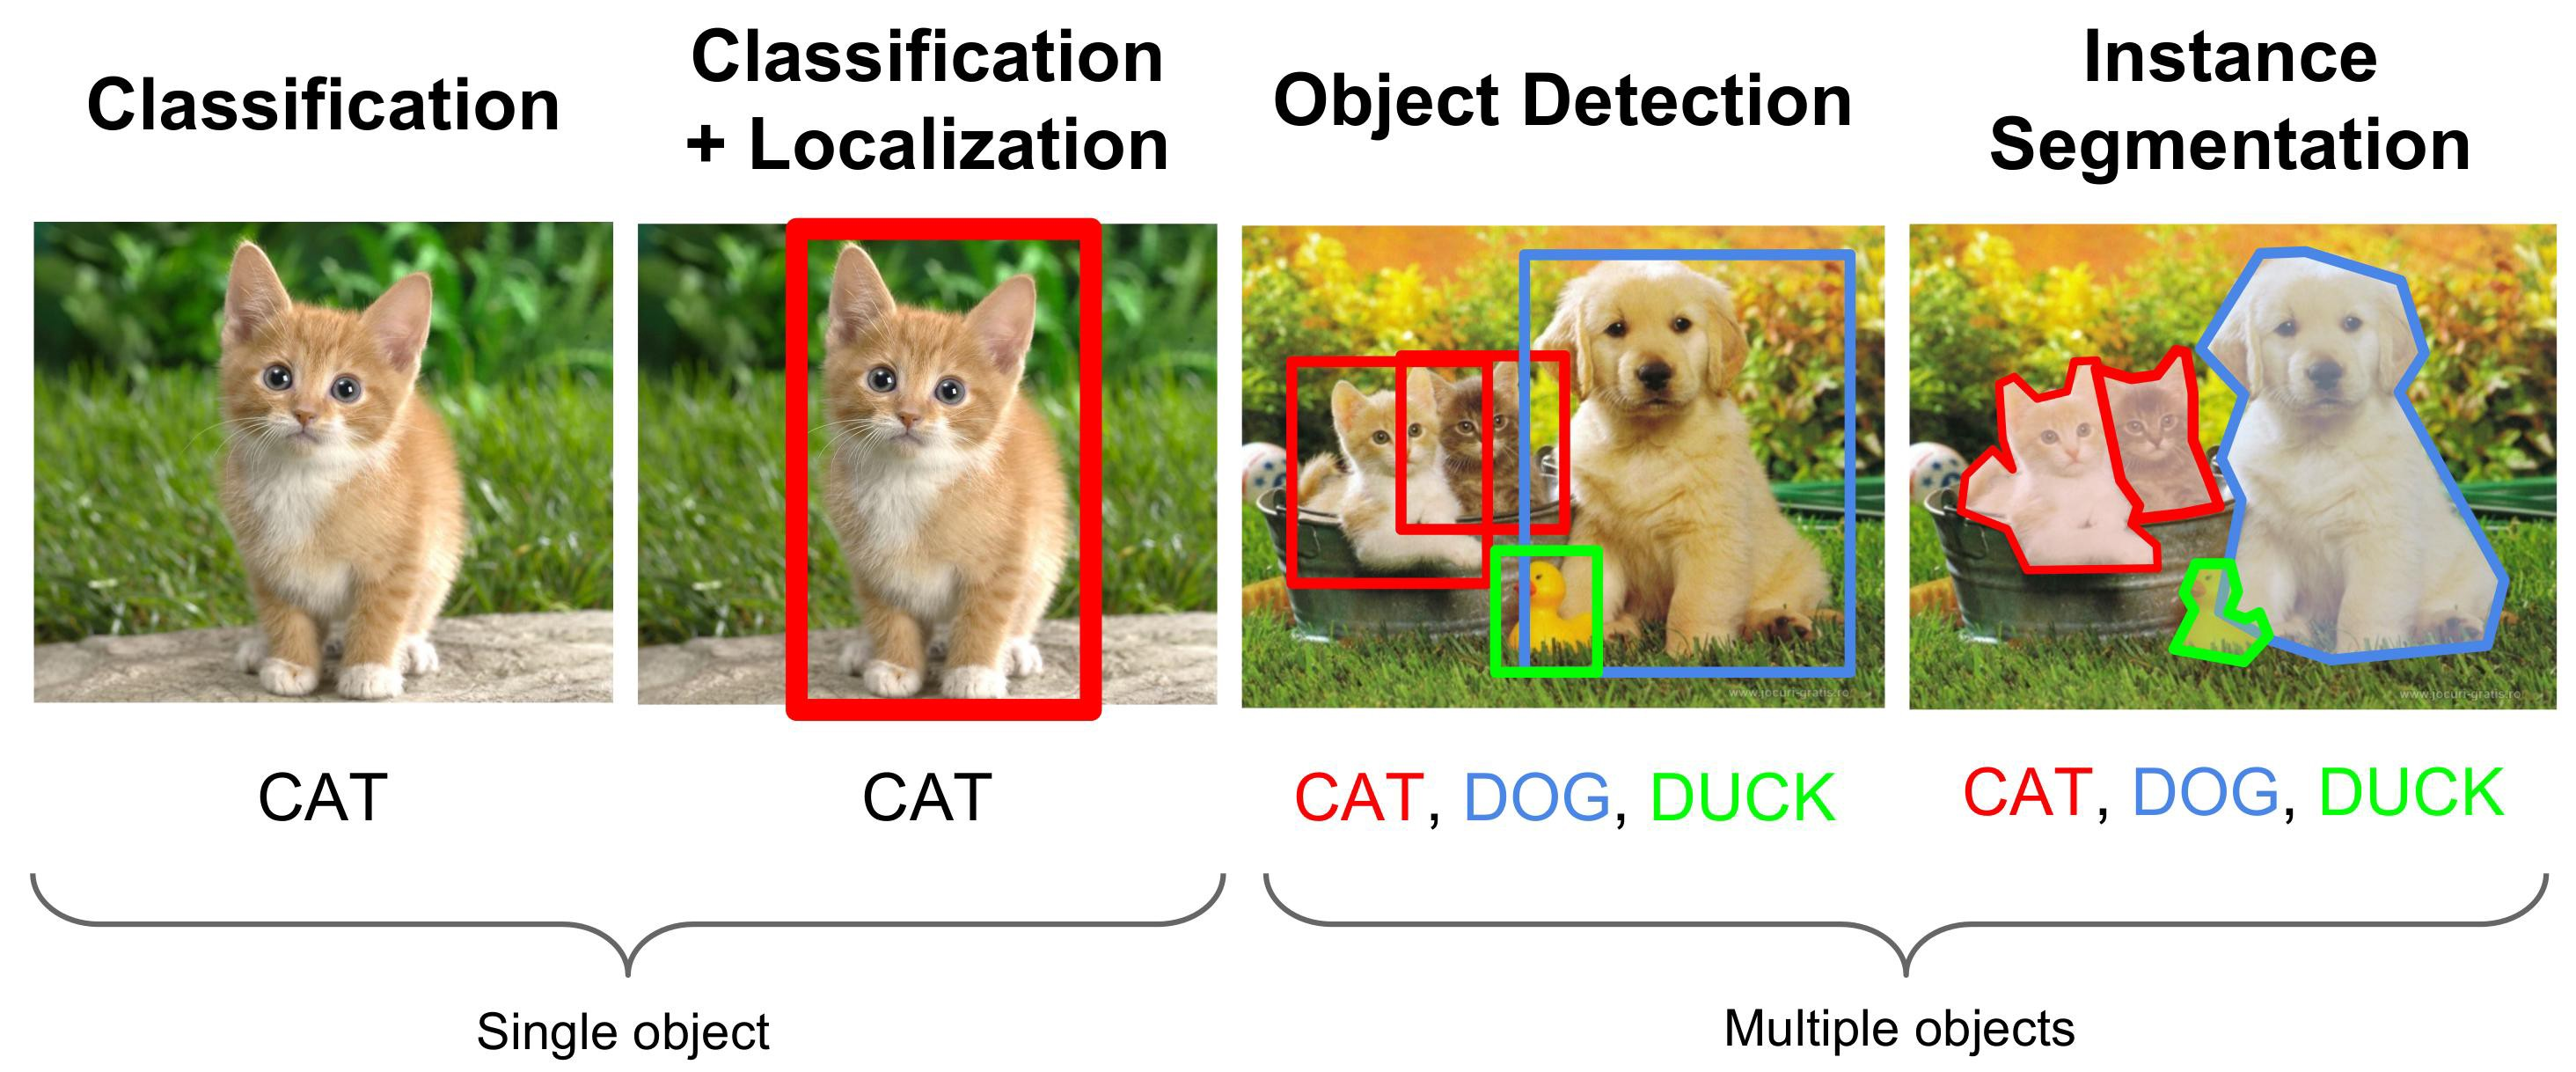
\includegraphics[width=13cm,height=5cm,]{./Images/ejemplotensorflow.jpg}
	\caption{Ejemplo de Clasificación de imagen de TensorFlow}
	\footnotesize Fuente: \cite{ejemplotensorflow}
	\label{tensorfl}
\end{figure}

Finalmente se empleo la iteración del punto más cercano \cite{grest2005nonlinear} el cual usa un enfoque de inicialización del esqueleto a través de fotogramas subsecuentes, clasificándolos con vértices y segmentos en un modelo 3D para este propósito.

La estimación de las poses humanas representan una problemática compleja de solucionar, el cual tuvo un largo trayecto hasta salir a la luz. La complejidad se centra en las múltiples limitantes, como las mascotas, los objetos del área, las personas de alrededor, la variación del escenario, los parámetros del cuerpo (el tamaño, longitud de las extremidades, torso y otras partes del cuerpo) y la iluminación.

Empleando las herramientas de seguimiento del Esqueleto, sensores de profundidad y sensores RGB, a medida que el tiempo corre, la necesidad de herramientas como los sensores va volviéndose obsoleta con el nacer de herramientas como PoseNet y OpenPose, que con el apoyo del Hardware mínimo necesario, son capaces de proporcionar la misma información con una calidad apenas inferior de seguimiento corporal.

\begin{figure}
	\centering
	\begin{subfigure}{.5\textwidth}
		\centering
		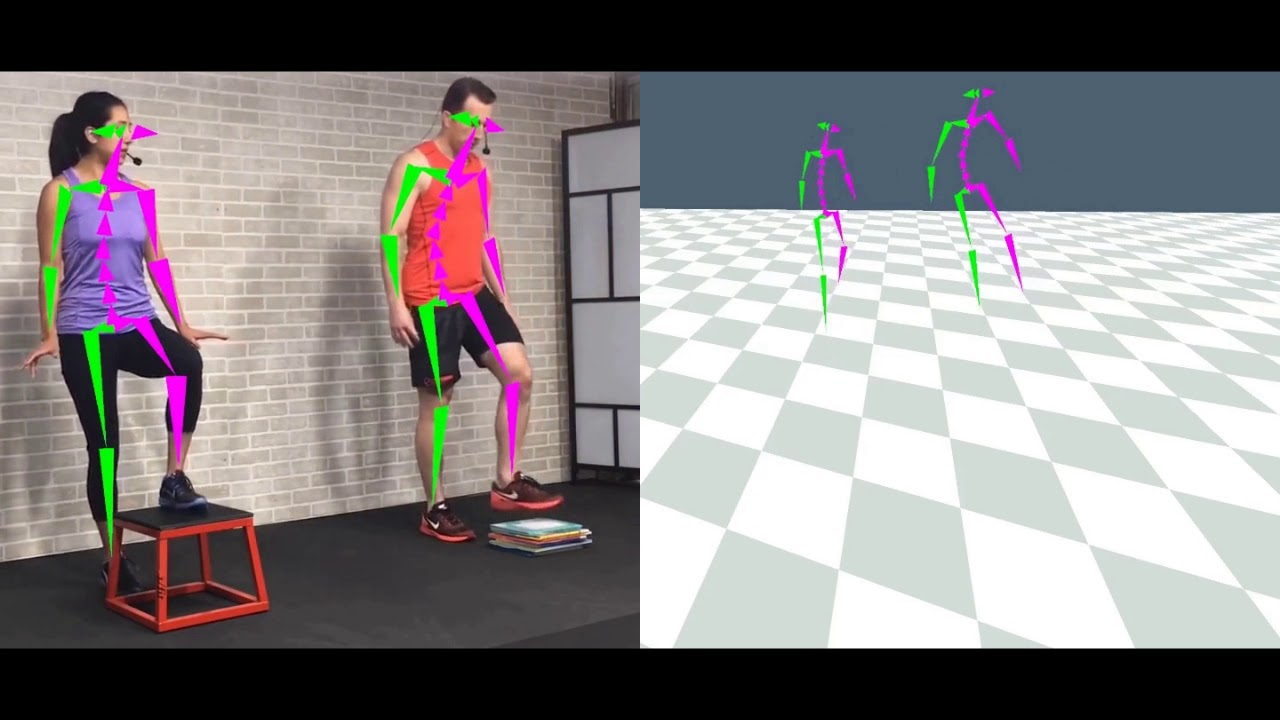
\includegraphics[width=8cm,height=7cm,]{./Images/examplebodytracking.jpg}
		\caption{Ejemplo 1}
		\label{bodyexa1}
	\end{subfigure}%
	\begin{subfigure}{0.5\textwidth}
		\centering
		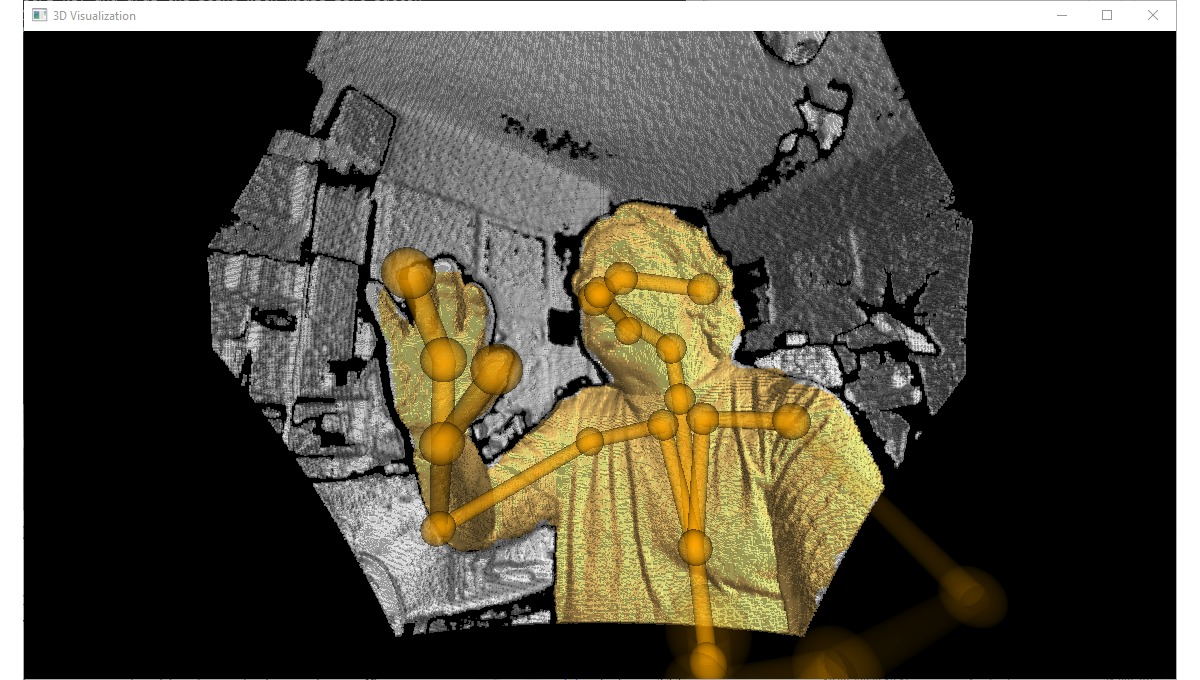
\includegraphics[width=8cm,height=7cm,]{./Images/examplekinect.jpg}
		\caption{Ejemplo 2}
		\label{bodyexa2}
	\end{subfigure}
	\caption{Ejemplos de Body Tracking}
	\footnotesize Fuente: \cite{examplebodytracking} \cite{examplekinect}
	\label{bodyexafigure}
\end{figure}

\subsubsection{Estimación de Poses}

La estimación de poses como su nombre indica, tiene la labor de estimar la pose de una persona a partir de modelos machine learning (ML) guardados en una base de datos, que proporcionan en ubicaciones especificas puntos clave que en su conjunto forman el esqueleto, además los datos sobre sus puntos se guardan como es explicado en el Análisis de Alternativas de PoseNet.

Se podría mencionar que su diferencia parte también de las palabras que lo conforman, Body Tracking/Capture Motion hace referencia a seguir el movimiento de una persona empleando Estimación de Pose, mientras que la Estimación de Poses hace referencia a marcar los puntos clave de una persona y construir un esqueleto de una persona \cite{oved2018real}.

\subsection{Skeletical Tracking}

Este fue una innovación brindada por el controlador Kinect al mercado comercial, Su demanda fue elevada en la época y hasta el día de hoy sigue siendo empleado, el reconocimiento de una persona desde cualquier angulo o distancia, tomando en cuenta su figura, tamaño, colo, cabello, ropa y el ambiente. Se emplea el escaneo de la imagen para reconocer puntos importantes del cuerpo que representan al cuerpo, tales como la cabeza, cuello, hombros, brazos, piernas y otros 10 a 20 puntos dependiendo la herramienta de reconocimiento que se emplee.


\begin{figure}[ht]
	\centering
	\begin{subfigure}{.5\textwidth}
		\centering
		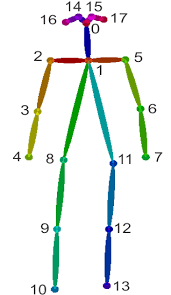
\includegraphics[width=4cm,height=6cm]{./Images/openposet1.png}
		\caption{Reconocimiento OpenPose Tipo COCO}
		\label{open1}
	\end{subfigure}%
	\begin{subfigure}{.5\textwidth}
		\centering
		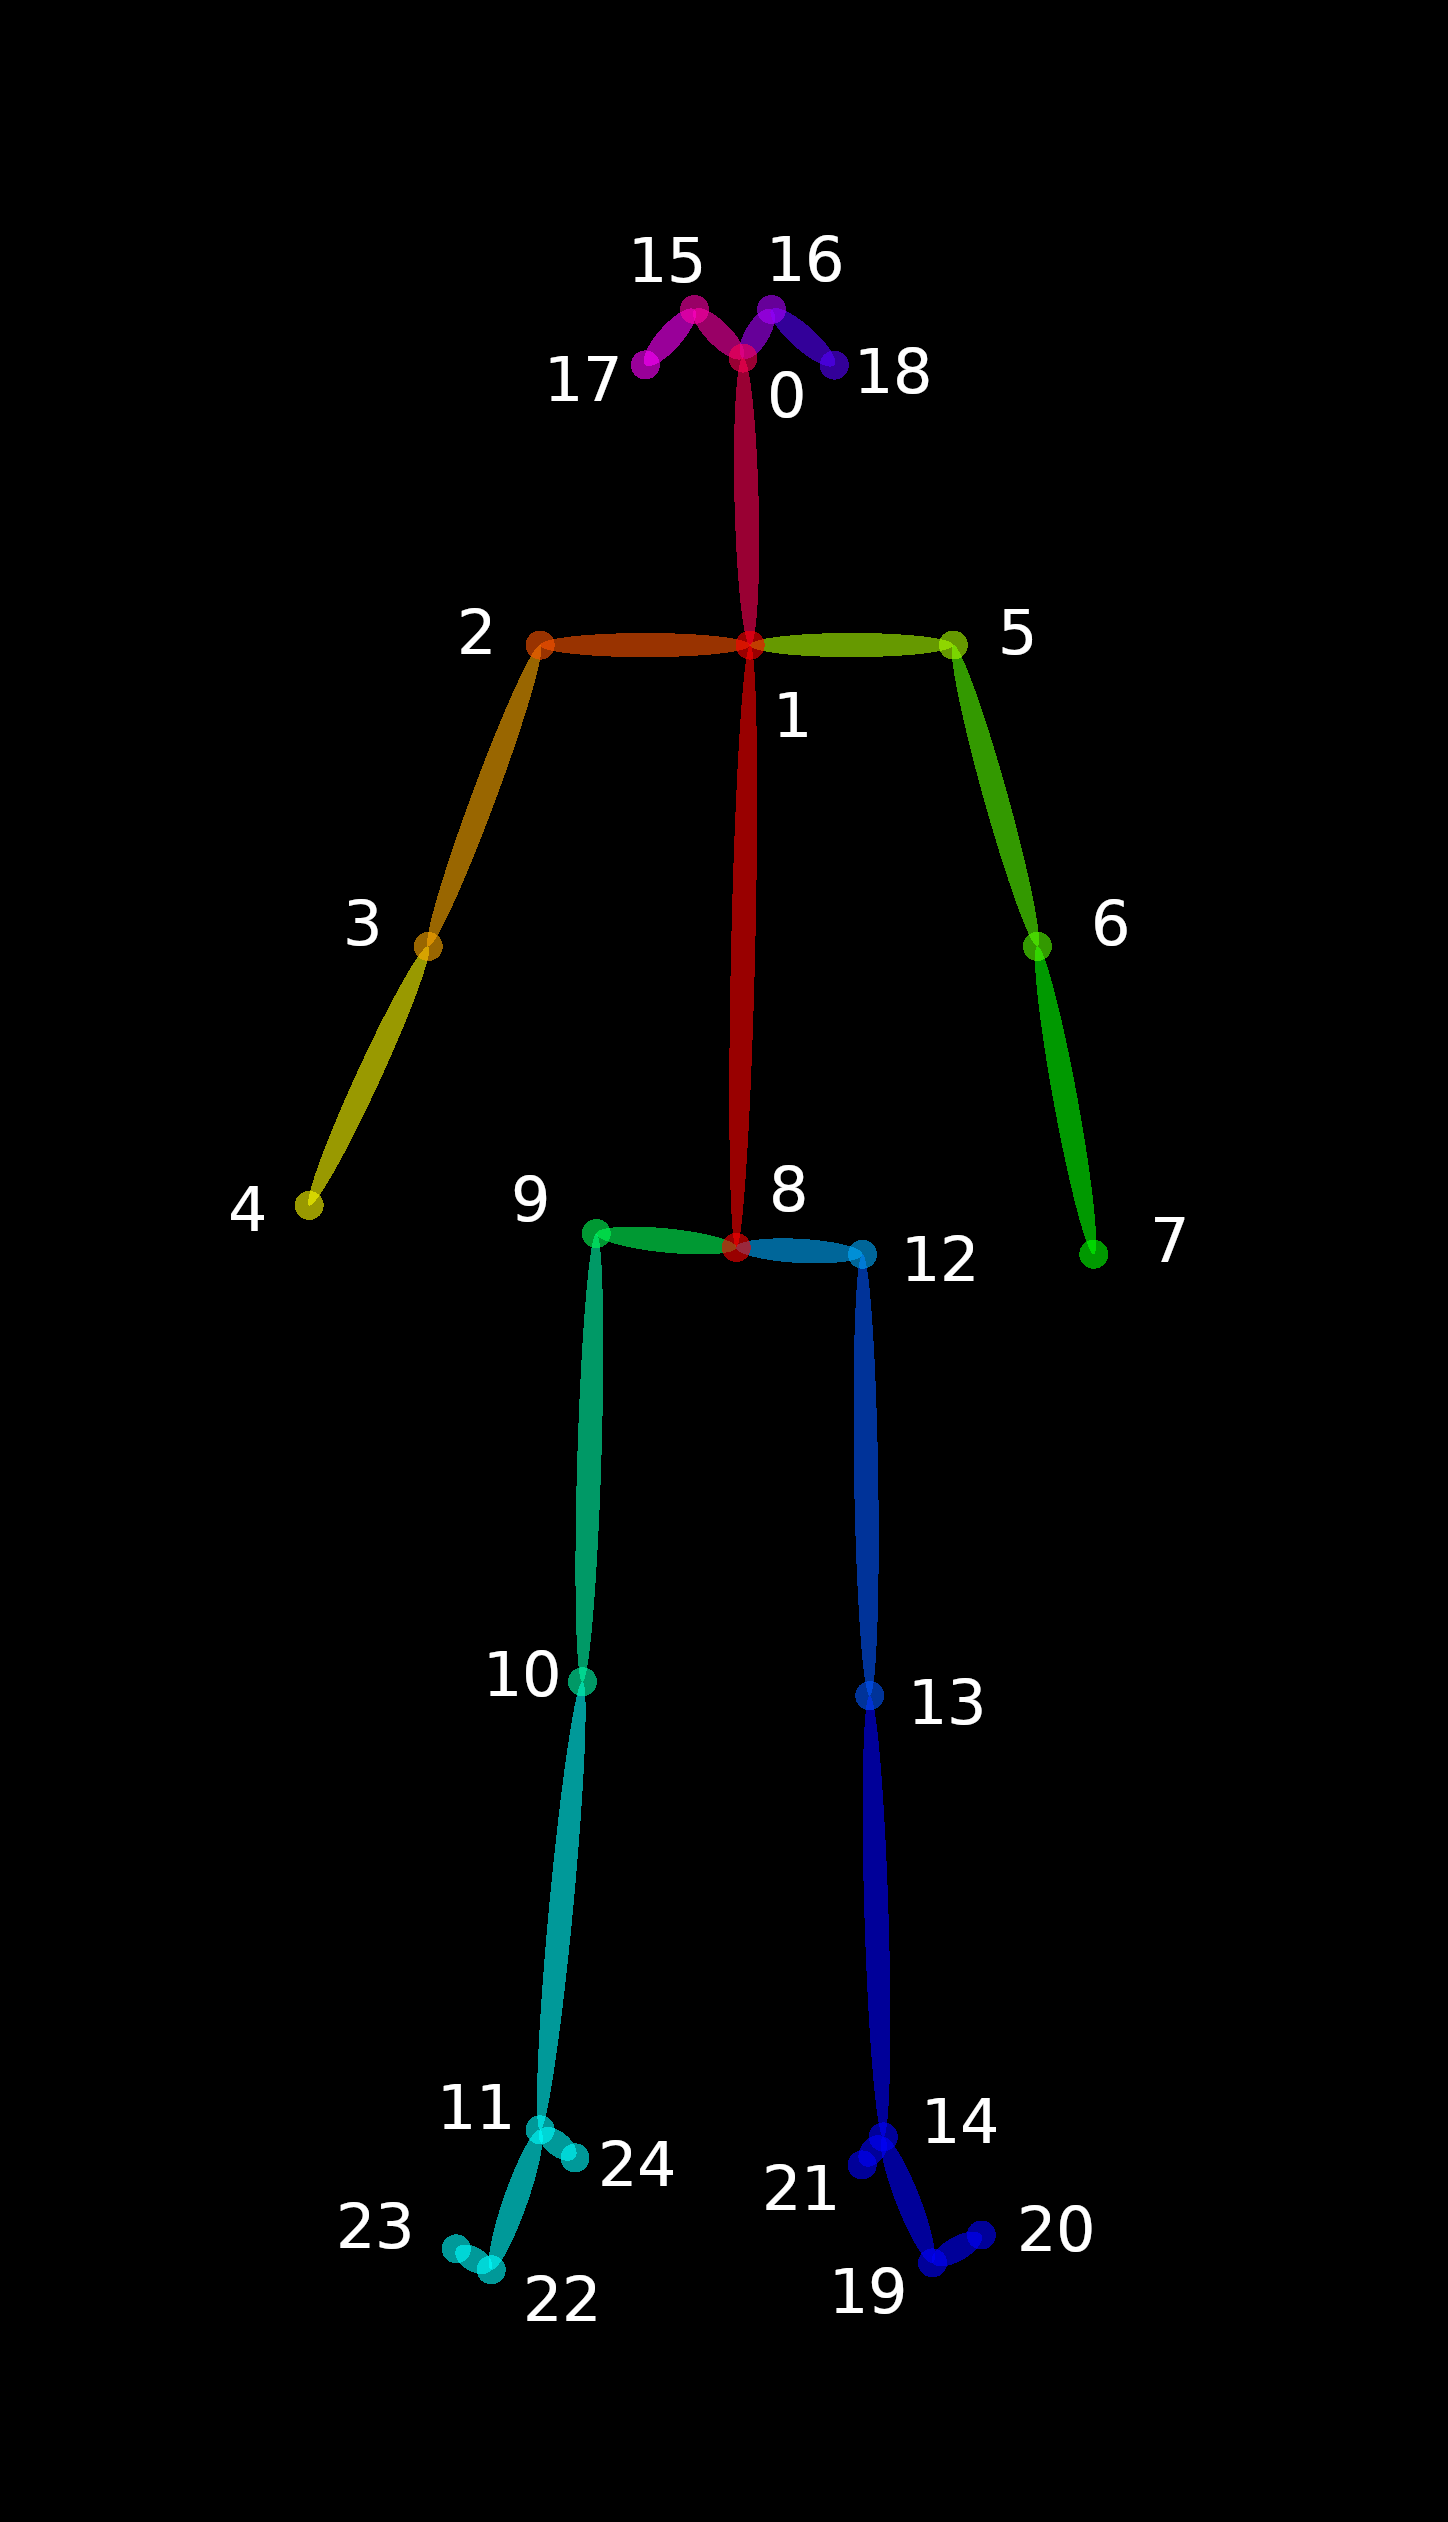
\includegraphics[width=4cm,height=6cm]{./Images/openposet2.png}
		\caption{Reconocimiento OpenPose Tipo BODY\_25}
		\label{open2}
	\end{subfigure}
	\caption{Diversos Tipos de Seguimiento al Esqueleto seleccionados por OpenPose para el desarrollo del proyecto}
	\label{exampleesqueletotrack}
	\footnotesize Fuente: OpenPose Models Image Output \cite{cao2017realtime} \cite{8765346}
\end{figure}

La herramienta seleccionada para el proyecto es OpenPose empleando este modelo de \href{https://github.com/CMU-Perceptual-Computing-Lab/openpose/blob/master/doc/output.md}{Formato de salida}, para los datos del seguimiento del esqueleto es emplear la flag write\_json para guardar la información dentro un JSON, el cual contiene un objeto de esqueleto de persona dentro, que contiene un vector pose\_keypoints\_2d con puntos 2D para localizar y detectar cada punto de unión x1,y1,c1,x2,y2,c2,.... Las coordenadas x y y en el rango de [0,1], [-1,1].

Además de la existencia de los vectores face\_keypoints\_2d, hand\_left\_keypoints\_2d y hand\_right\_keypoints\_2d, análogos a pose\_keypoints\_2d, los cuales debido a la masiva carga de memoria que requieren y la falta de ella (mínimo 4GB de Memoria dedicada estimada, contando solo con 2GB en el equipo proporcionado) serán ignorados, pero empleando pose\_keypoints\_2d.

Como dato, los vectores análogos body\_keypoints\_3d, face\_keypoints\_3d,
hand\_left\_keypoints\_2d y hand\_right\_keypoints\_2d (si se habilitase), en vez de 
x1,y1,c1,x2,y2,c2,..., el formato sería x1,y1,z1,c1,x2,y2,z2,c2,..., donde c sería 1 o 0 dependiendo si la reconstrucción 3D es exitosa.

Se empleara el modelo BODY\_25 de Caffe, para mostrar el esqueleto, que consiste en mostrar 25 puntos del esqueleto, cada uno con su conexión en los siguientes puntos clave:

\begin{table}[t]
	\begin{center}
		\begin{tabular}{| c | c | c | c | }
			\hline Pos. & Punto Clave & Pos. & Punto Clave \\ \hline
			0 & Nariz&13 & Rodilla Izquierda \\ \hline
			1 & Cuello &14 & Tobillo Izquierdo \\ \hline
			2 & Hombro Derecho& 15 & Ojo Derecho \\ \hline
			3 & Codo Derecho & 16 & Ojo Izquierdo \\ \hline
			4 & Muñeca Derecha & 17 & Oreja Derecha \\ \hline
			5 & Hombro Izquierdo & 18 & Oreja \\ \hline
			6 & Codo Izquierdo & 19 & Dedo Gordo Izquierdo \\ \hline
			7 & Muñeca Izquierda & 20 & Dedo Meñique Izquierda \\ \hline
			8 & Cadera Central & 21 & Talón Izquierdo \\ \hline
			9 & Cadera Derecha & 22 & Dedo Gordo Derecho \\ \hline
			10 & Rodilla Derecha & 23 & Dedo Meñique Derecho\\ \hline
			11 & Tobillo Derecho & 24 & Talón Derecho \\ \hline
			12 & Cadera Izquierda & 25 & Escenario \\ \hline
		\end{tabular}
		\caption{OpenPose Output JSON Content, Which are Given X, Y and C values}
		\footnotesize Fuente:\cite{8765346}
	\end{center}
\end{table}


En cuanto al resultado, este se puede guardar en formatos estándar (JSON, XML, PNG, JPG,...), existen suficientes herramientas de uso libre para leerlos, por tanto cargar los datos y cargar las imágenes, no debería representar un desafió.

\section{Base Teórica}

\subsection{Cámara y Desambiguación}

Una cámara se define como un dispositivo que permite el registro y reproducción de imágenes. A través del tiempo, se desarrollaron muchos tipos de cámara, por tanto es necesario determinar el tipo de cámara del cual se dispone para la elaboración del proyecto, siendo el selecto la cámara Web. Sin embargo, en la mayoría de proyectos relacionados al Body Tracking, se menciona el termino Depth of Field (DOF), mención a una cámara de profundidad de campo.

La cámara web es un modelo pequeño de una cámara digital conectada a una computadora. Tiene la capacidad de capturar imágenes y transmitirlas a través de Internet. Un punto importante es que pueden ser empleadas para el desarrollo de aplicaciones y programas de cierta índole. 


\subsubsection{Depth of Field (DOF)}

La profundidad de campo es el producto del deseo de producir una imagen más clara del objeto o escenario deseado. Normalmente, una cámara debe enfocar su lente para tener mayor precisión, por tanto, se adjuntaron formas para ajustar el lente. Actualmente, se desarrollaron sistemas automáticos para el ajuste del lente, los cuales incluyen la medición de la distancia al objetivo, empleando esta para ajustar el lente y obtener mayor claridad \cite{madsen2000depth}. 

\subsubsection{Sensores RGB-D} 

Es el termino dado al conjunto de sensores RGB y Depth (de profundidad).Los sensores de RGB y profundidad son una adición a los dispositivos como Kinect, PlayStation Camera y otros. 
\\El sensor de profundidad cumple la función de proyectar luz infrarroja y un sensor infrarrojo. 

Divide su funcionalidad en dos pasos, la proyección de rayos de luz infrarroja, los cuales rebotan en el ambiente en el que se encuentra y posteriormente son detectados por el sensor de infrarrojo. Esta información es decodificada y enviada al usuario para poder emplearla como se lo estime.
\\
RBG es un modelo de colores basado en la obtención de un color empleando una mezcla entre otros colores, todas ellas con los colores primarios, que son el rojo, verde y azul. 
El sensor RBG analiza el escenario que tiene en frente, determinando la cantidad de luz que requiere la producción de una imagen de calidad, optimiza y ajusta la velocidad de obturación, apertura y sensibilidad de captura de luz. 
Se encarga de analizar cada pixel del Frame y crear una imagen meticulosa.
\\
En el desarrollo del proyecto, no se empleara un sensor de profundidad, ya que una cámara Web no lo tiene equipado.

La funcionalidad del sensor RGB-D es combinar la información colectada por el sensor infrarrojo y el sensor RGB, proporcionan datos de color y profundidad a cada pixel en cada Frame que analiza. Dentro de la memoria del Kinect, existen patrones de referencia, que poseen colores y profundidades ya conocidas, que facilitan la estimación del escenario que lo necesite\cite{litomisky2012consumer}.  
\begin{figure}[t!]
	\centering
	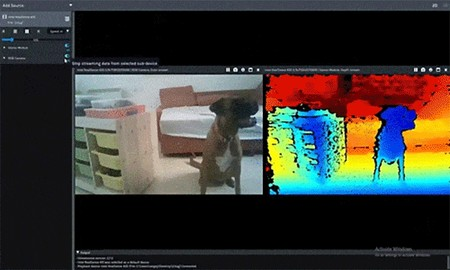
\includegraphics[width=10cm,height=6cm,]{./Images/RGBandDepth.jpg}
	\caption{Ejemplo de Visión de una Cámara con sensores RGB-D}
	\footnotesize Fuente: \cite{RGBandDepth}
	\label{RGBandDepth}
\end{figure}


\subsection{Inteligencia Artificial (IA)}

Una faceta importante del proyecto, es la estimación de poses, elemento producto de la Inteligencia Artificial y Machine Learning, si bien, es explicado en la sección de PoseNet.
\\
La inteligencia artificial (IA) es una rama de la ciencia de computación, que se define como "Un programa que en un mundo arbitrario, no se las arregle peor que un humano"\cite{dobrev2012definition}. 
Esta definición se somete a muchos factores, para empezar requiere de asumir tres factores importantes.
El primer factor es que cualquier dispositivo de calculo puede ser modelado por un programa. El segundo factor es que el IA es un dispositivo que permite ingresar información de afuera y dar una respuesta de acuerdo a ello. El tercer factor es asumir que la IA, al estar en contacto con el mundo este recibe información que da una respuesta interactiva con el mundo. Se asume que el mundo en que se encuentre será influenciado por la IA\cite{dobrev2012definition}. El mundo se considera como el ambiente con el que la IA tiene interacción, aquel que proporciona los valores que la IA procesará y aquel que reaccionará a las acciones y/o valores de salida de la IA, en un proceso de emisión y recepción continuo.

\subsubsection{Machine Learning (ML)}

El aprendizaje de la máquina o Machine Learning es ua rama de la ciencia de computación dirigida en algoritmos Computacionales diseñada para emular la inteligencia humana, a través del aprendizaje del mundo que lo rodea.

Los modelos ML ganan popularidad debido a su capacidad de proporcionar resultados y conocimientos de un tipo especifico en escenarios similares a los que ha entrenado, pero nunca antes visto. Los modelos ML provee información relevante sobre los datos relacionados a lo que se requiere, traduciendo los datos de entrada, en datos que se desean obtener. Por ejemplo, un médico, para diagnosticar a un paciente con un síntoma tan común como fiebre, requerirá de un extenso conocimiento en enfermedades que tienen este síntoma y basándose en todo su conocimiento teórico, indagara en información que pueda relacionar con la fiebre, especificando otros problemas o falta de ellas que tenga y llegará a una conclusión sobre que enfermedad padece \cite{murdoch2019interpretable}.

Una versión simplificada es decir que Machine Learning emplea algoritmos para clasificar y filtrar la información recibida, aprender de ella, guardarla y tomar una decisión basándose en lo aprendido. 

\subsubsection{Deep Learning (DL)}

El aprendizaje profundo o Deep Learning es una subrama de Machine Learning que se basa en el uso de Neural Network, empleando numerosas capas y nodos para el aprendizaje, que en conjunto a toda la base de datos previa da lugar las decisiones en las que se basa.

El Deep Learning utiliza múltiples capas de decisión, siendo el dato de ingreso interpretado por el logaritmo en diferentes niveles, cada uno repercute en el anterior y produce un aprendizaje basado en intento y error para aprender, corrigiendo los datos de salida de cada capa para llegar a una respuesta cada vez más aproximada a la deseada.
Una diferencia importante entre Machine Learning y Deep Learning, es que, Machine Learning en general mejora con el tiempo, pero requiere de corrección de vez en cuando, si se desvía de los resultados que se buscan.En cambio, Deep Learning determina si su propia predicción es correcta haciendo uso de su red neuronal, no requiere de intervención.
\\
En el desarrollo del proyecto se hace mención al modelo CAFFE y COCO, los cuales son parte fundamental en el proyecto, ya que estas son los modelos de Deep Learning empleados para el Body Tracking.

\subsubsection{Modelo DL CAFFE}

El modelo CAFFE es un Framework opensource trabajado con las librerias C++ y CUDA para Deep Learning, tiene interfaces en Command Line, Python y MathLab, incluye soporte en problemas con el modelo, tiene referencias, demos y herramientas para poder usarlo, además de la caracteristica de usarse con CPU y GPU\cite{jia2014caffe}.

Además de poseer una comunidad abierta a ampliar el desarrollo y trabajar con la herramienta, ventaja caracteristica del codigo open source. 
El modelo CAFFE ofrece el poder definir modelos, optimizar opciones para el desarrollo y pre-entrenar para poder realizar el aprendizaje.

En la sección del proyecto, CAFFE realizo sus estudios para poder guardar Dataset de miles de cuerpos humanos, otorgándole puntos clave para formar el esqueleto. 
La herramienta OpenPose selecta hace uso de la CMU Panoptic Dataset, que junto a  sus miles de miles de esqueletos 3D permite estimar la pose humana, produciendo el Modelo BODY\_25 visto previamente en la figura \ref{open1}.

\subsubsection{Modelo DL COCO}

EL modelo COCO es un Dataset reciente del año 2014, desarrollado para el reconocimiento de objetos en el contexto requerido, a través de la obtención de imágenes complejas que contengan la información requerida en su estado natural.
En su mayoría, posee objetos reconocibles por niños pequeños, tiene 2.5 millones de etiquetas en mas de 300000 imágenes.

En el contexto, el modelo COCO posee miles de imágenes relacionadas a la identificación del cuerpo humano y la construcción de su esqueleto, marcando con etiquetas sus puntos claves del cuerpo y la confiabilidad de esos datos\cite{lin2014microsoft}.

\subsubsection{Neural Network}

Neural Network inicialmente es inspirado por la compleja red de neuronas del cuerpo humano, el cual transmite información, ordenes a través de impulsos eléctricos, donde miles de millones de conexiones existen, con ese fin\cite{wang2003artificial}. 
\\

Formalmente, el modelo de Neural Network consiste en un set de unidades Computacionales y un set de conexiones de una vía unidas. A través del ingreso de datos, las unidades Computacionales lo examinan y computan, generando una activación como dato de salida. La activación atraviesa la conexión que tiene la unidad Computacional con otra unidad y procede a examinarlo y computarlo para generar otra activación. 
Este proceso se repite, con el fin de aumentar el llamado peso que determina la influencia que se obtiene al examinar y computar el valor recibido, dependiendo el objetivo, mientras mayor o menor termine siendo el peso en las conexiones a medida que se computan las activaciones en las unidades Computacionales, mayor efecto tendrá en el dato de salida. 
Un ejemplo de ello se observa en la figura \ref{neuralnetwork} \cite{gallant1993neural}, donde los círculos representan unidades Computacionales, las flechas las conexiones, los valores los pesos, ingreso de datos es el 1 y el dato de salida es 0. El 0.73, 0.79 y 0.69 es el resultado de una Activación después del primer computo.
\\
Esta herramienta es empleada por OpenPose y PoseNet para el entrenamiento de las herramientas de estimación de pose, que lo utilizan para que con los Dataset de miles de imágenes que sirven como imágenes de ingreso y sus etiquetas, puedan ser analizadas por extensas capas de unidades Computacionales que evaluaran cada imagen y proporcionaran pesos, que a mayor peso, mayor precisión en la estimación de pose tendrá.
\begin{figure}[t!]
	\centering
	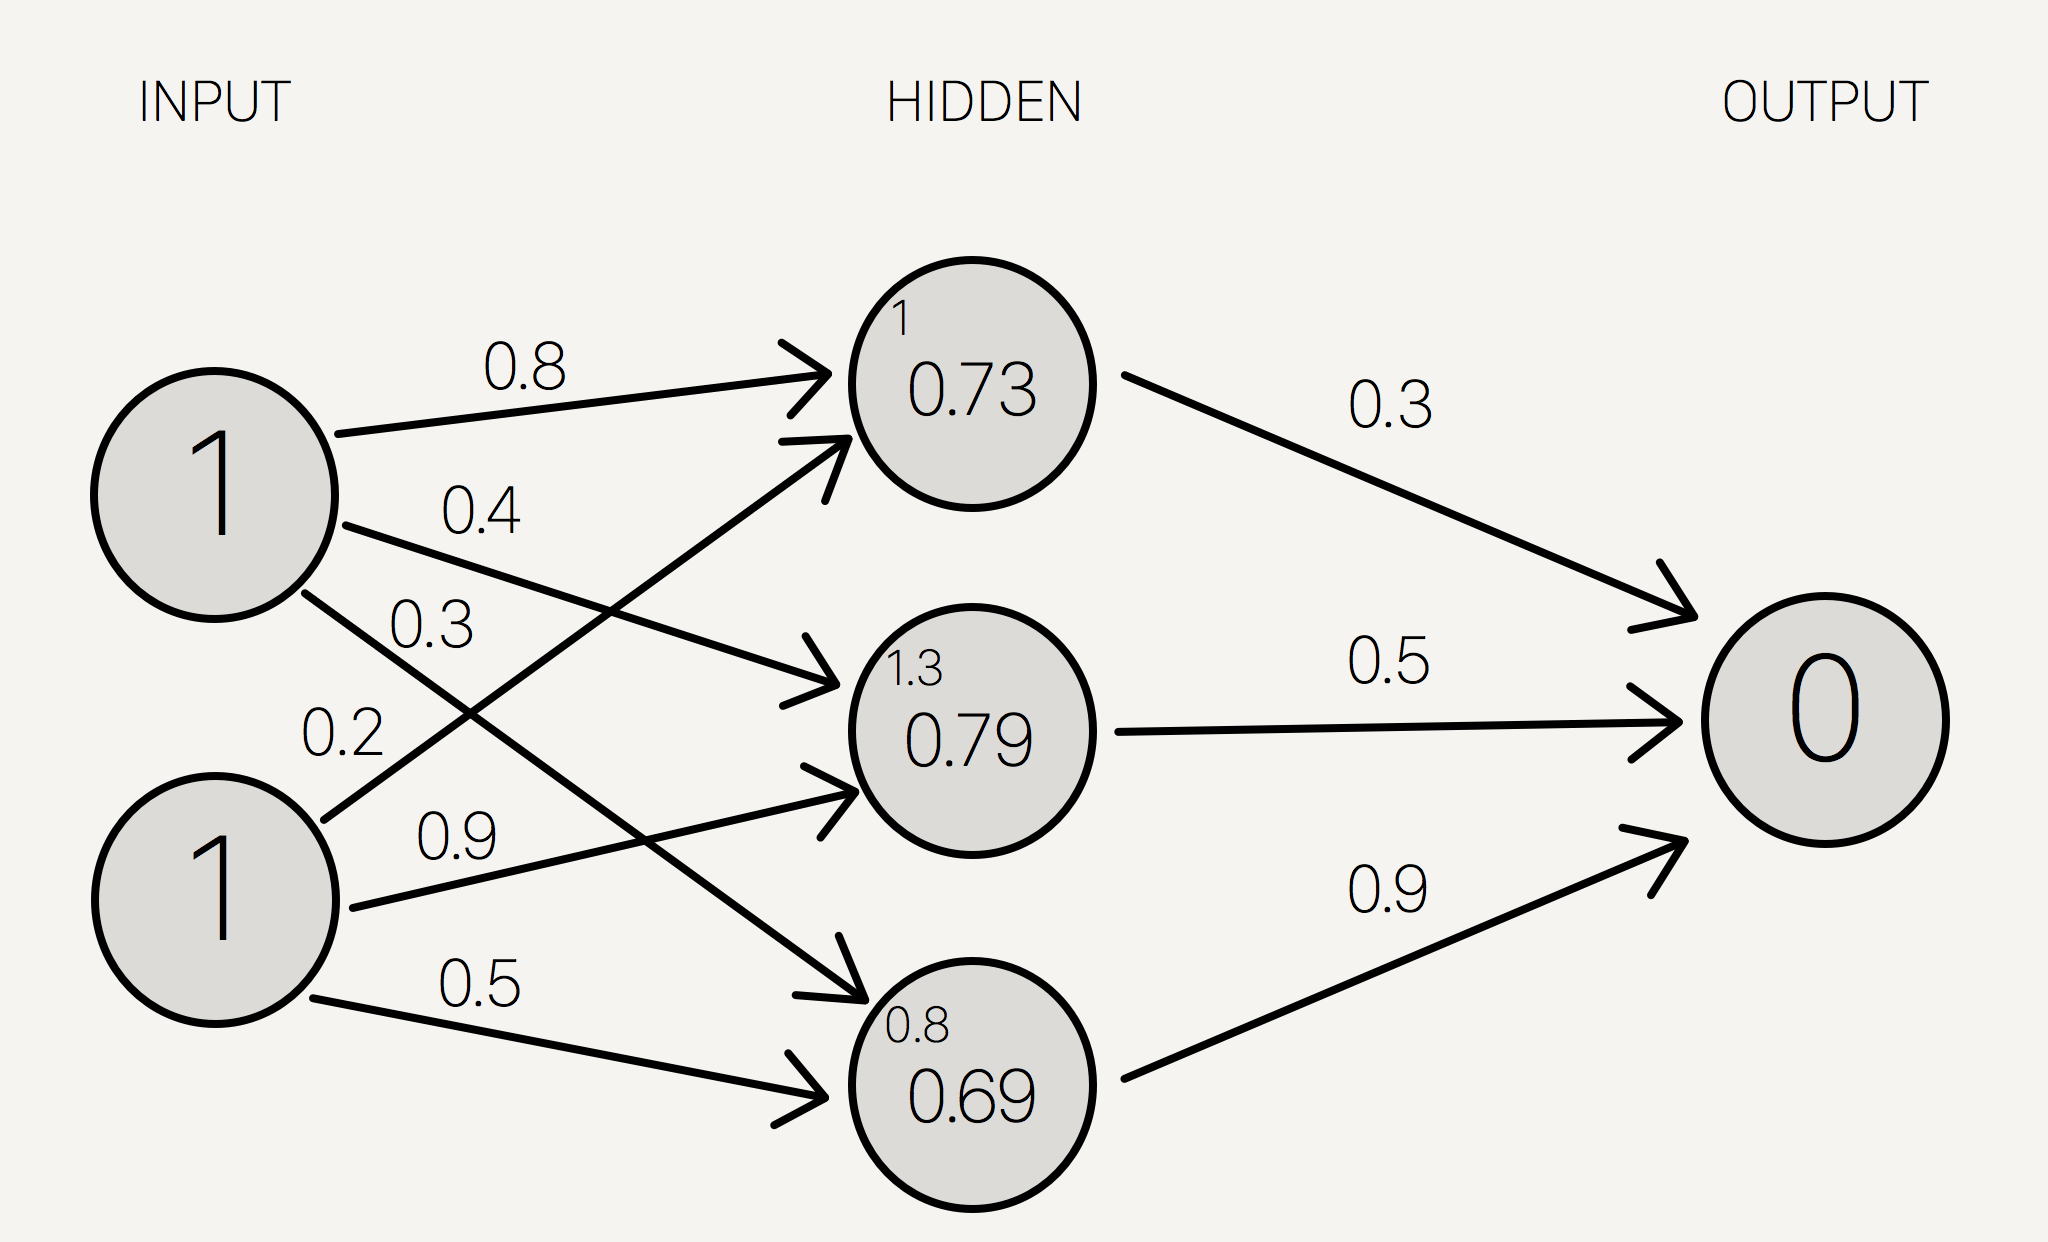
\includegraphics[width=11cm,height=5cm,]{./Images/neuralnetwork.png}
	\caption{Ejemplo de Neural Network}
	\footnotesize Fuente:\cite{8765346}
	\label{neuralnetwork}
\end{figure}